\chapter{Analysis}
\label{Analysis_chapter}

Since MadGraph needs as input parameter the mass of the heavy neutrino, two signals were simulated. One signal was made with a value of 5.0 GeV for the heavy neutrino mass, while the other assumed 
this mass to have a value of 70.0 GeV. 

In order to study the performance of a variable to reduce the backgrounds, histograms of this variable were made for each signal and background. These histograms are then placed on the same graphic 
and each one is normalized to the corresponding luminosity. This normalization makes possible to compare the performance of the variable among them. The luminosity of the accelerator is given by 50 $fb^{-1}$. If 
each histogram is not normalized it will depend on the size of the simulated sample. In these graphics the bins of one background are located above the corresponding bins of the other background. 
Thus, the total background is given by the curve of the background at the top. The background uncertainty is represented by a dashed line at the top of the background histograms. These kind of 
graphics are called stacked plots. The graphs shown here include just the W+jets and DY+jets backgrounds because these are very large compared to the 
$t\overline{t}$ background, and reducing them is already a difficult task.

The analysis started by studying the distribution of different variables after the preselection cuts and some cuts on three variables: number of jets, taus and b-jets. The first variable studied 
was $\vec{E_T^{miss}}$, and its stack plot is shown in Figure \ref{MET_bjets}. The graphic shows that the amount of background is much larger than both signals. Moreover, the distribution of the 
variable is similar for the signals and backgrounds. This implies that a cut on this variable would reduce the background in a similar way as it would reduce the signal. Thus, it is not possible 
to find an optimal cut value of MET.

 \begin{figure}[h] 
 \centering
 \caption{$E_T^{miss}$ distribution for the signal and backgrounds}
 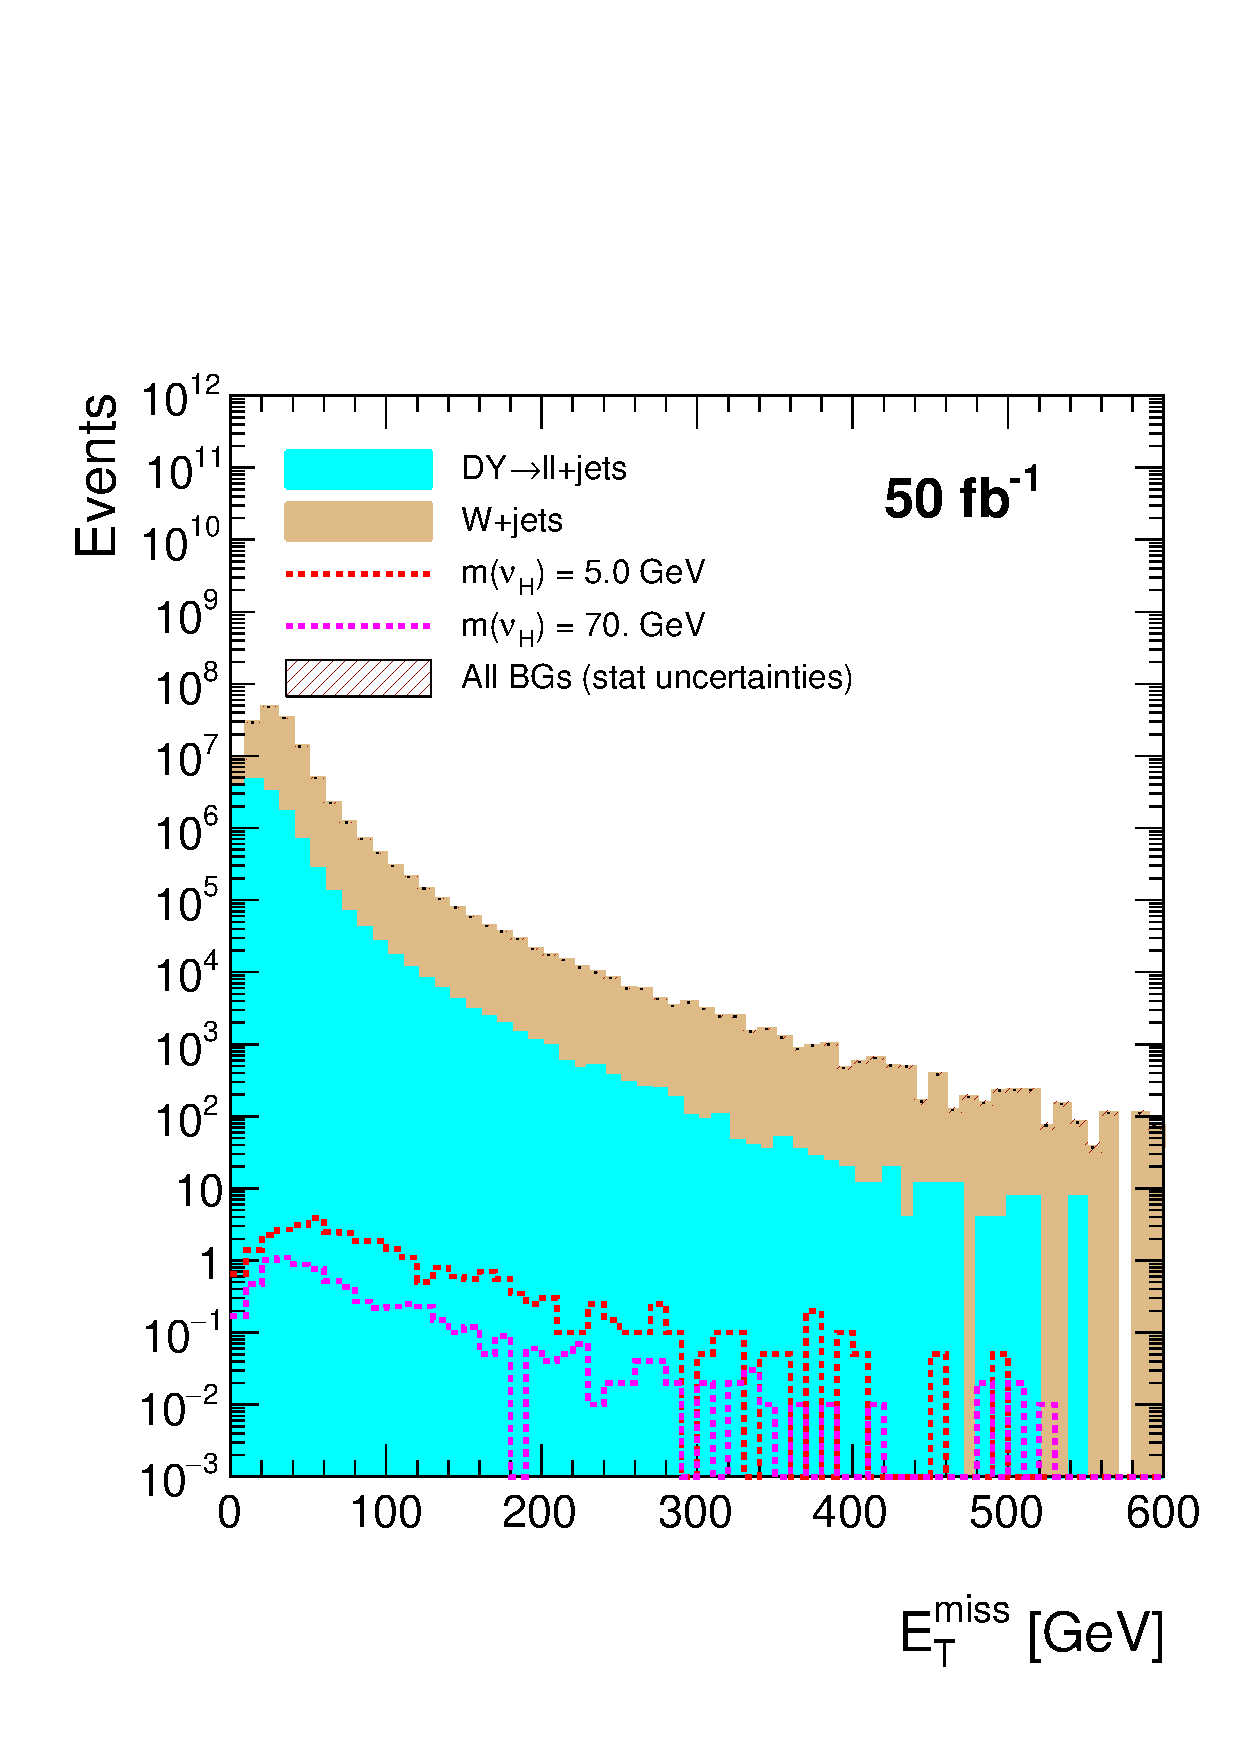
\includegraphics[width=0.8\textwidth]{./Capitulos/Analysis/AfterBJets/MET_MET_20} 
 \label{MET_bjets}
 \end{figure}
 
Next, we studied the distribution of more variables in order to be able to find the optimal cut values. The variables are $H_T$, diJetMass and the $p_T$ of the tau, and they are shown in the 
Figures \ref{HT_bjets}, \ref{diJetMass_bjets} and \ref{taupt_bjets}. It is possible to see that the distribution of these variables is similar for the signals and backgrounds. As a consequence, 
a set of optimal values of cuts on these variables that allows to reduce the background below the signal can not be determined.
 
 
\begin{figure}[h]
\centering
\begin{subfigure}{.5\textwidth}
  \centering
  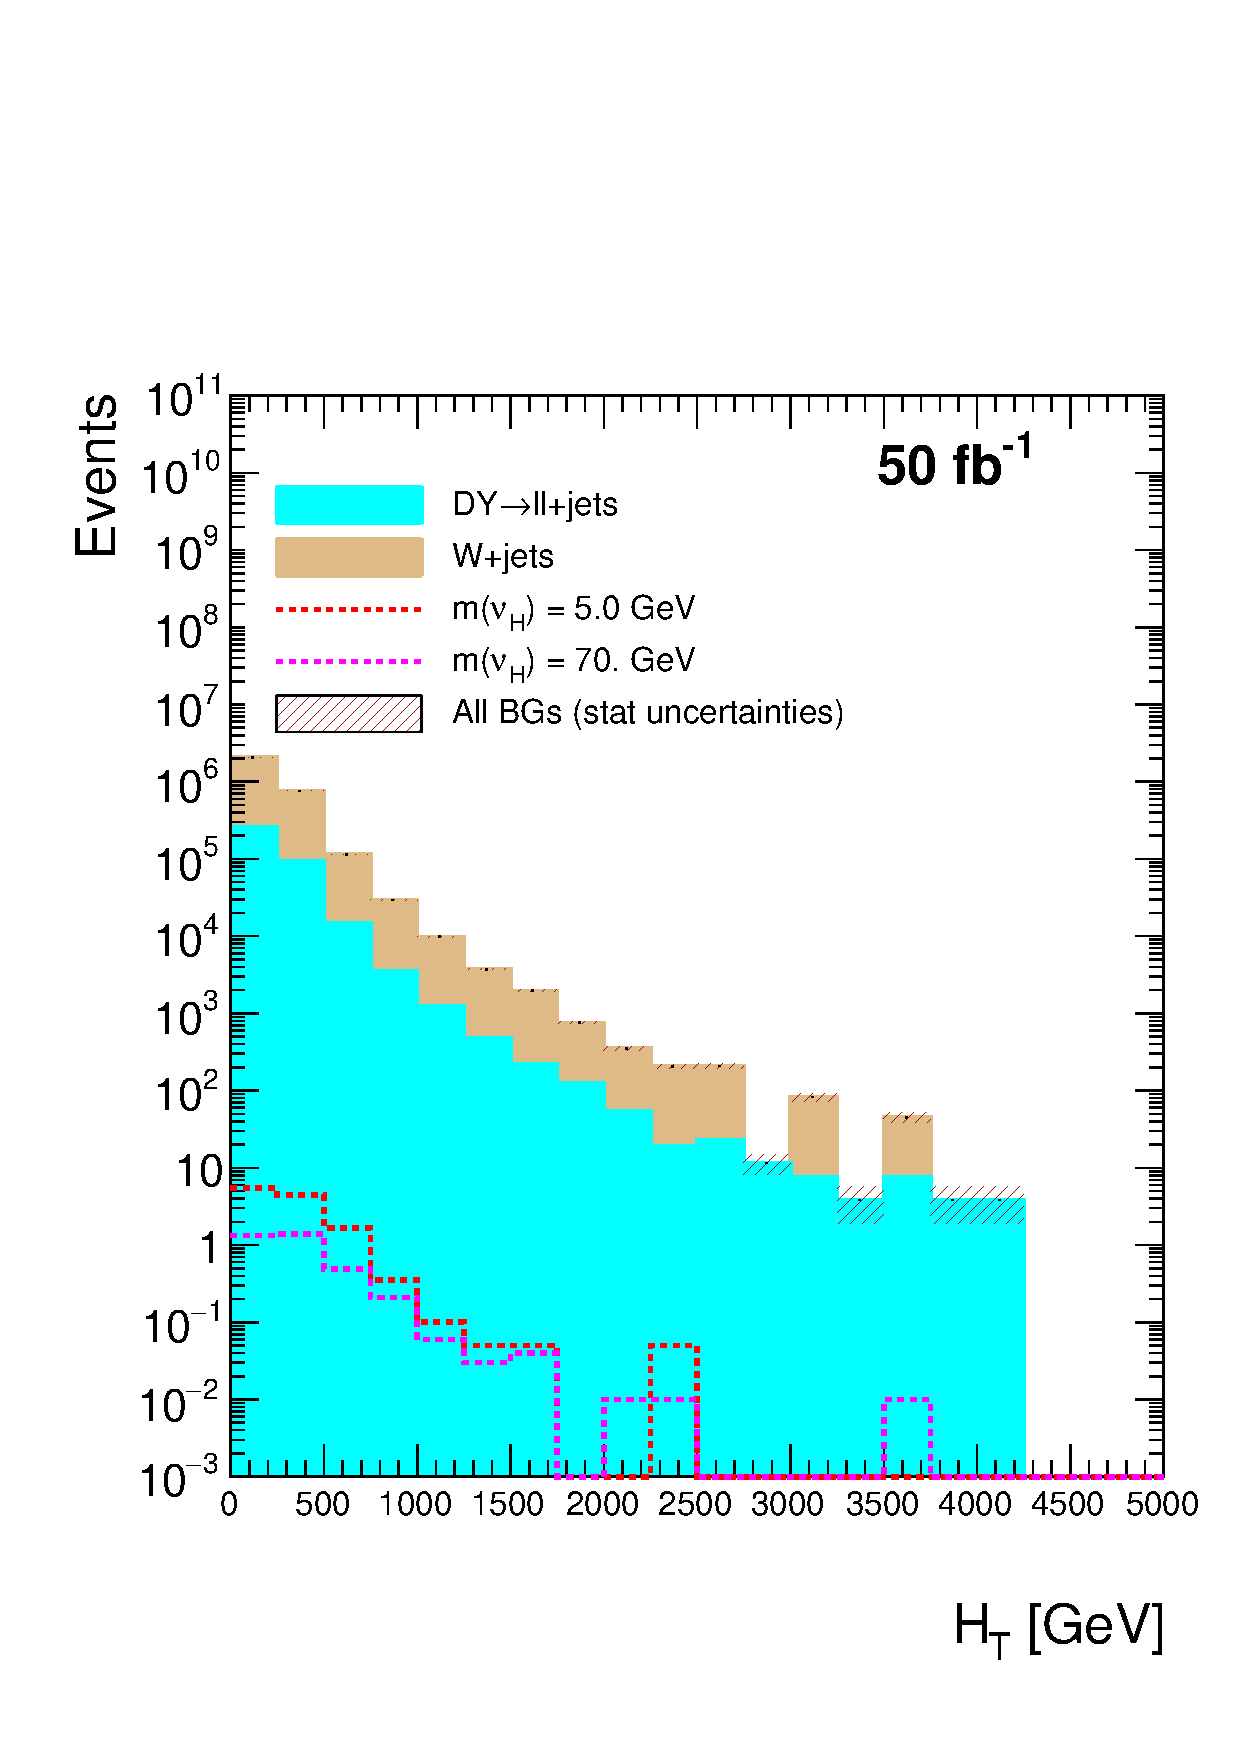
\includegraphics[width=1.1\linewidth]{./Capitulos/Analysis/AfterBJets/HT_MET_20}
  \caption{$H_T$ distribution for the signal and background}
  \label{HT_bjets}
\end{subfigure}%
\begin{subfigure}{.5\textwidth}
  \centering
  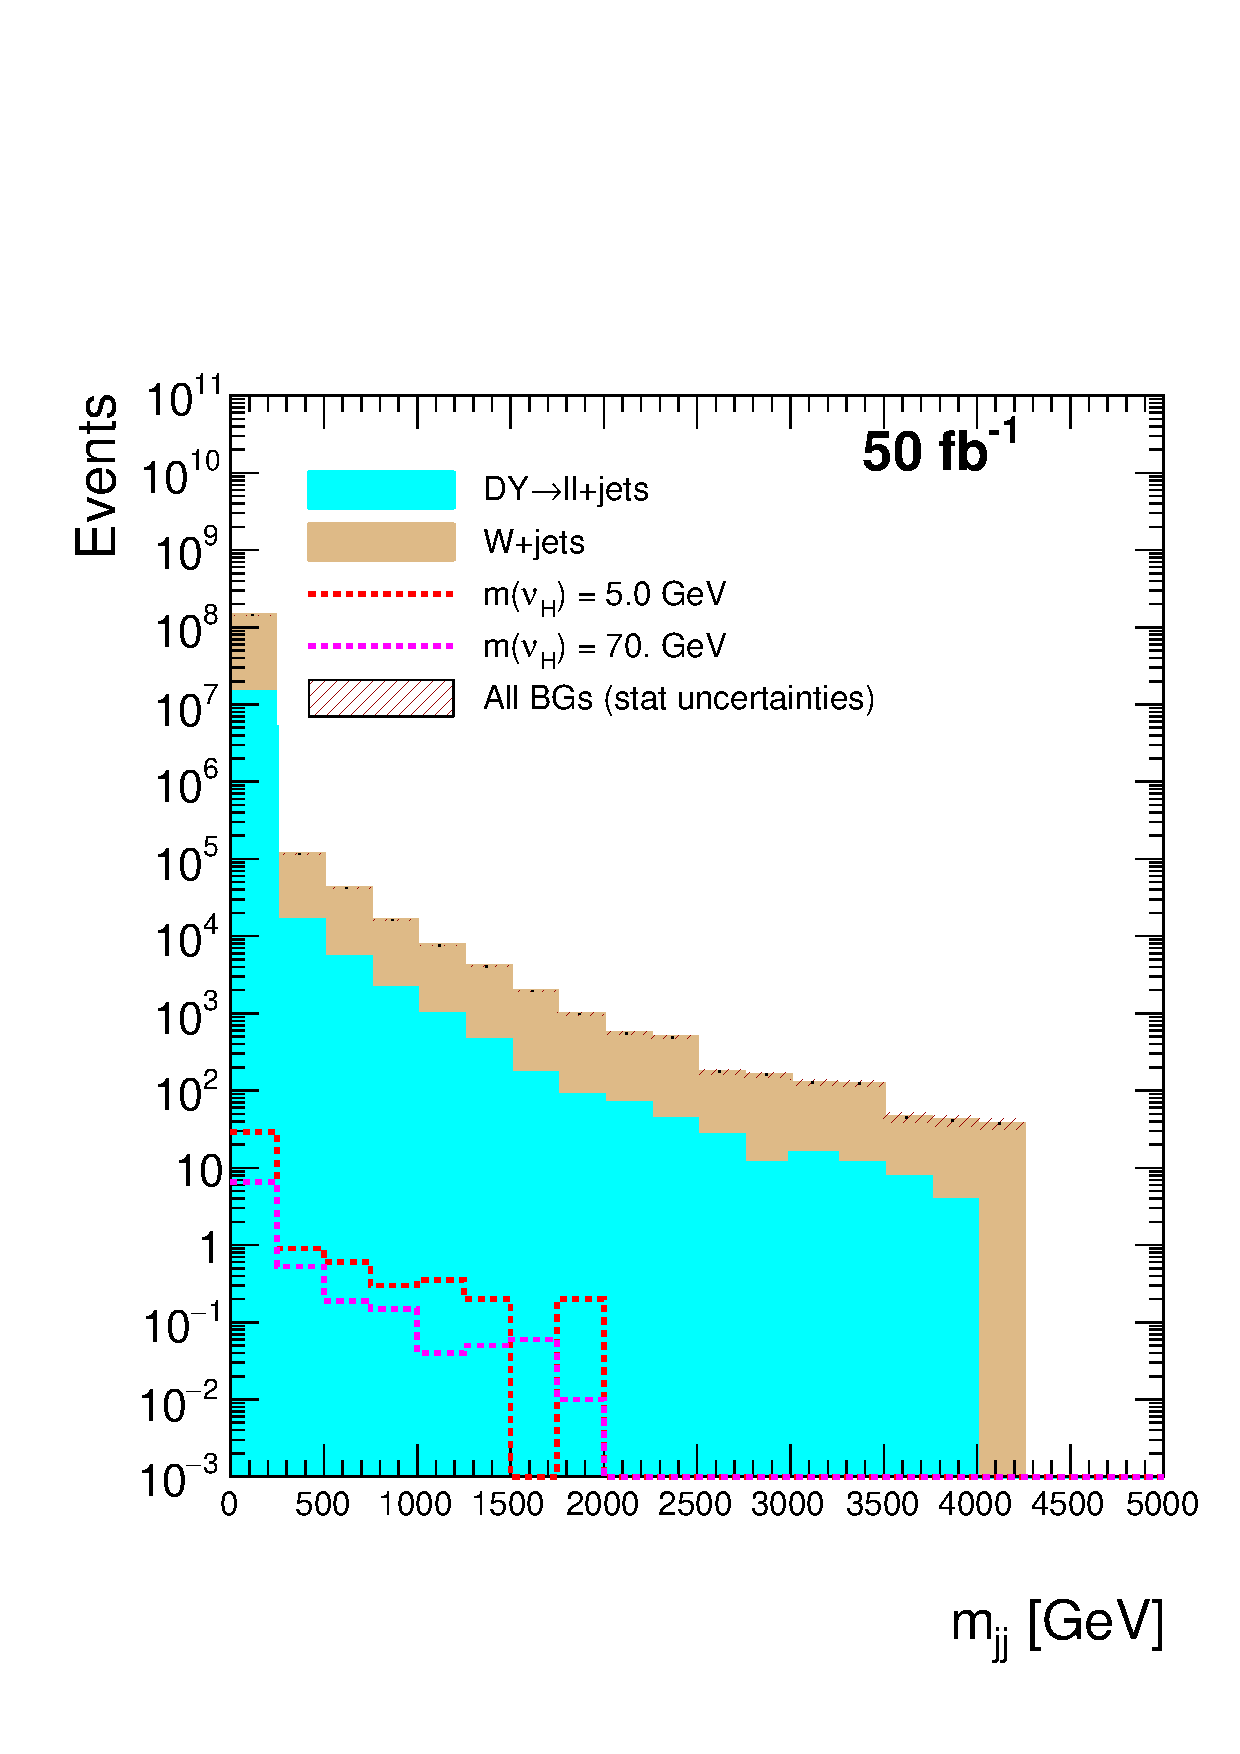
\includegraphics[width=1.1\linewidth]{./Capitulos/Analysis/AfterBJets/mjj_MET_20}
  \caption{diJetMass distribution for the signal and background}
  \label{diJetMass_bjets}
\end{subfigure}
\begin{subfigure}{.5\textwidth}
  \centering
  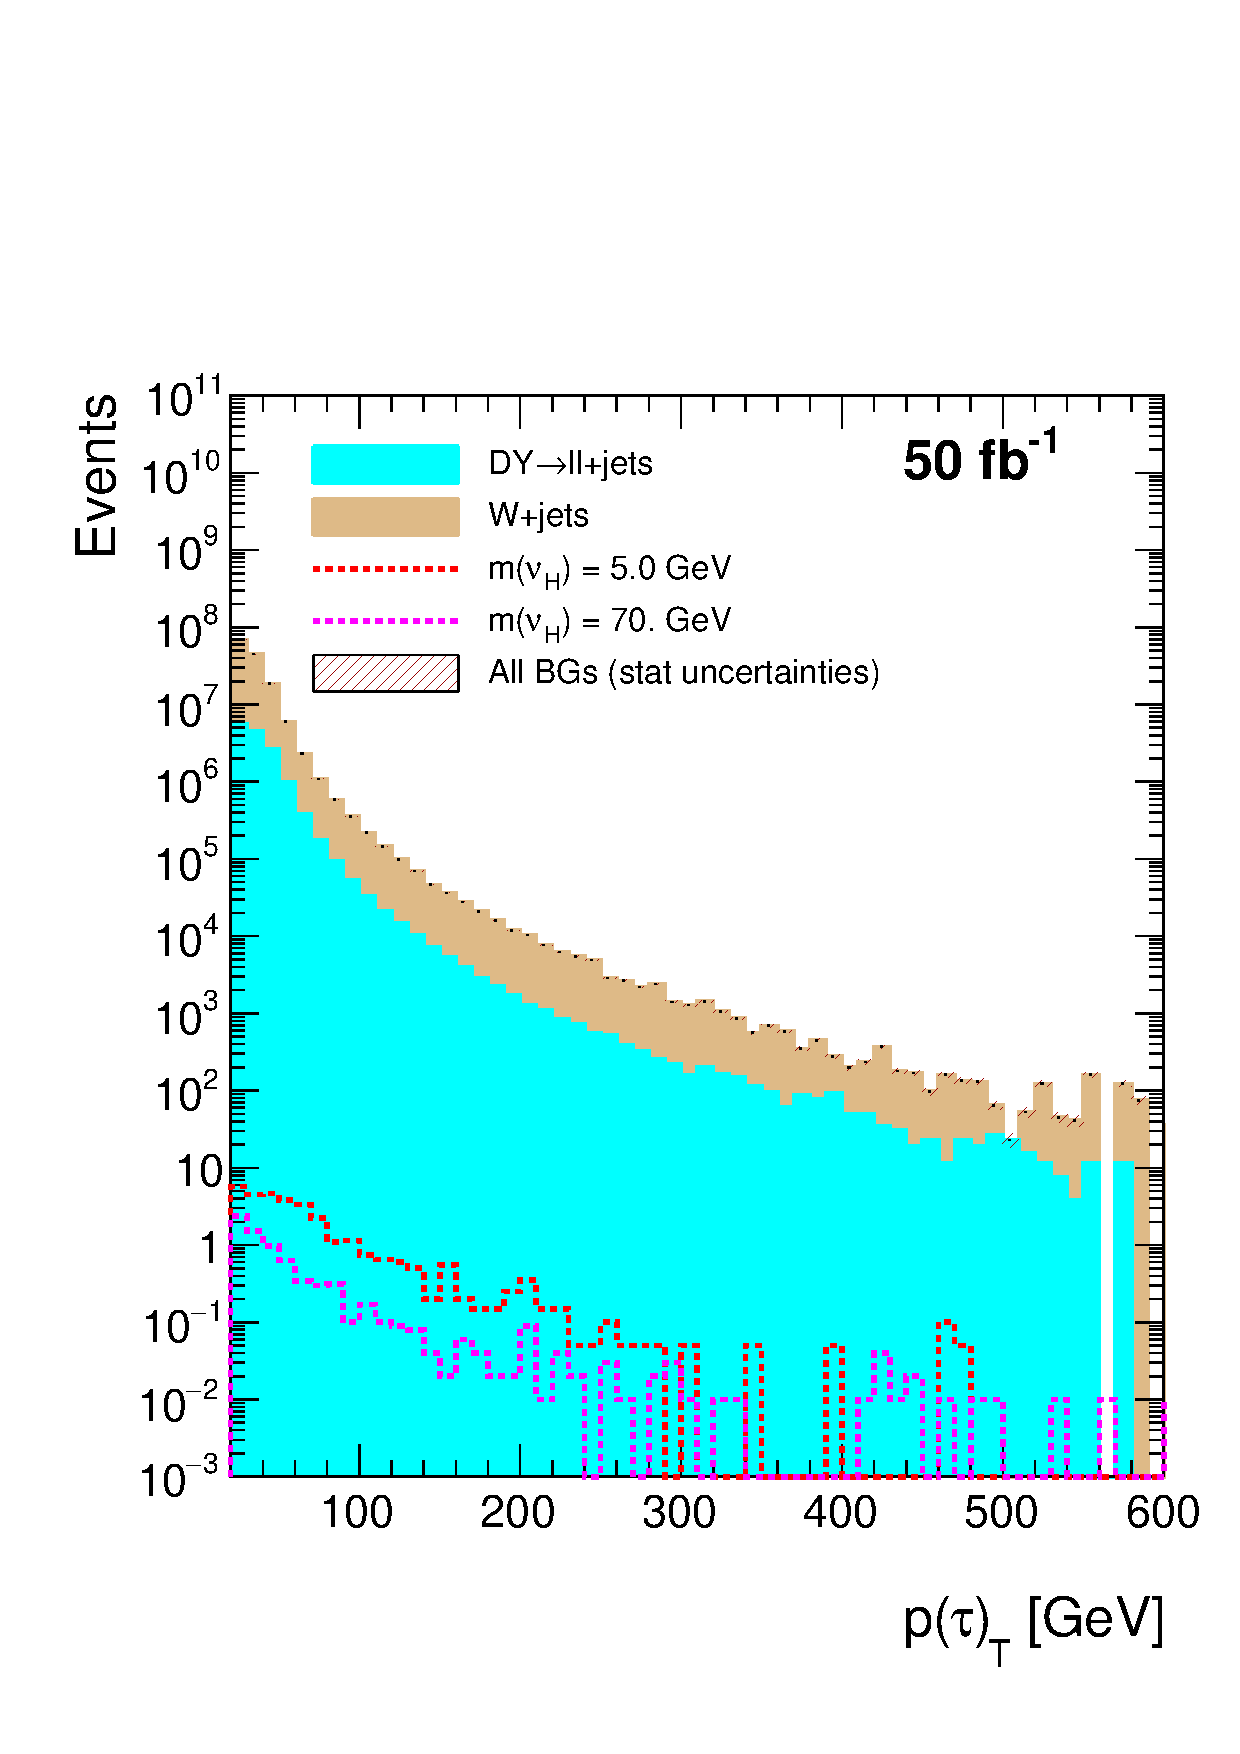
\includegraphics[width=1.1\linewidth]{./Capitulos/Analysis/AfterBJets/TauPt_MET_20}
  \caption{$p_T(\tau)$ distribution for the signal and background}
  \label{taupt_bjets}
\end{subfigure}
\caption{Distribution of diferent variables after cuts in the number of jets, taus and b-jets}
\label{Variables_bjets}
\end{figure}
 
 Then, all the cuts mentioned in the Chapter \ref{Event_selection_criteria_chapter} are imposed. These cuts include the ones related to the VBF process and the results are showed in the following 
 graphics. The variables $H_T$, diJetMass and $p_T(\tau)$ are shown is the figures \ref{HT_VBF}, \ref{diJetMass_VBF} and \ref{taupt_VBF}. In these graphics, one can see that after imposing all the 
 cuts the amount of signal and backgrounds reduces drastically. 
 
 \begin{figure}[h]
\centering
\begin{subfigure}{.5\textwidth}
  \centering
  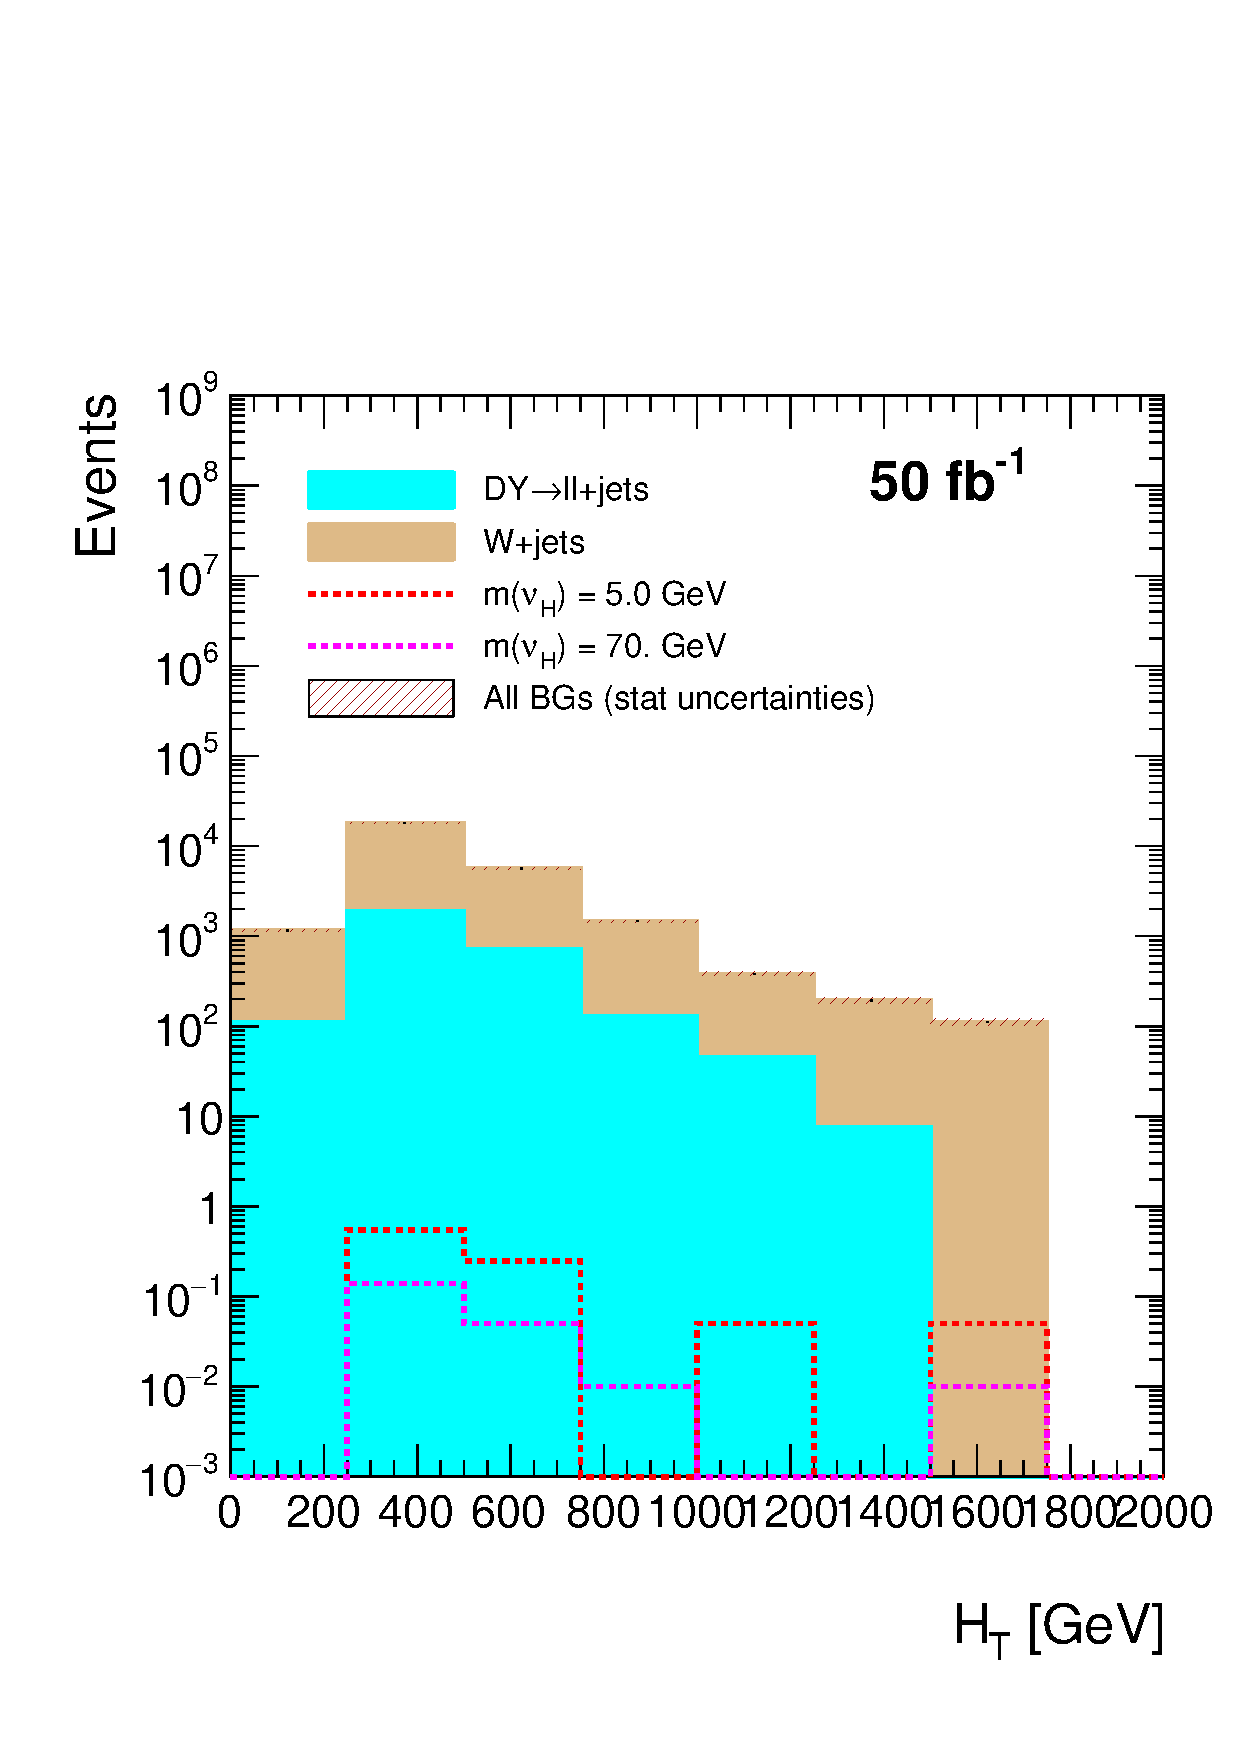
\includegraphics[width=1.1\linewidth]{./Capitulos/Analysis/AfterVBFCUTS/HT_MET_20}
  \caption{$H_T$ distribution for the signal and background}
  \label{HT_VBF}
\end{subfigure}%
\begin{subfigure}{.5\textwidth}
  \centering
  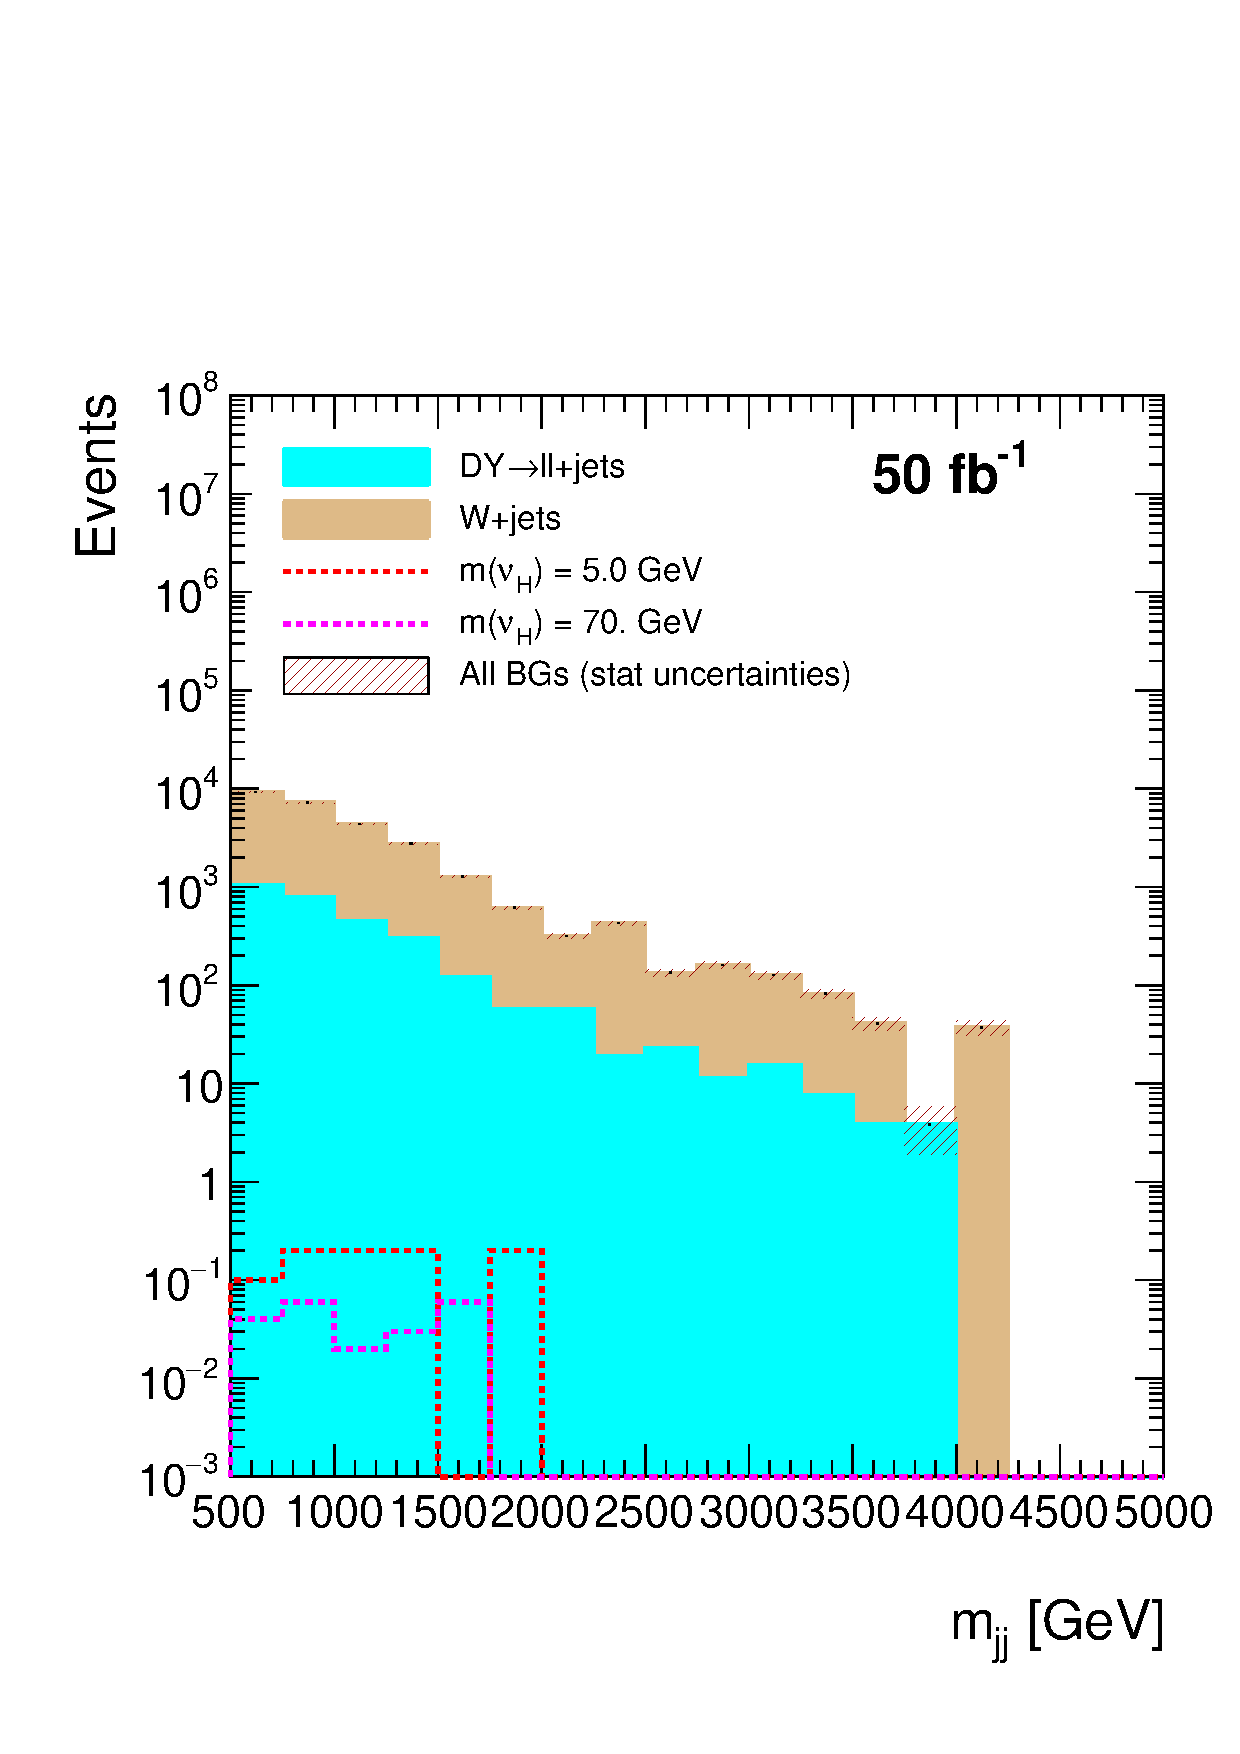
\includegraphics[width=1.1\linewidth]{./Capitulos/Analysis/AfterVBFCUTS/mjj_MET_20}
  \caption{diJetMass distribution for the signal and background}
  \label{diJetMass_VBF}
\end{subfigure}
\begin{subfigure}{.5\textwidth}
  \centering
  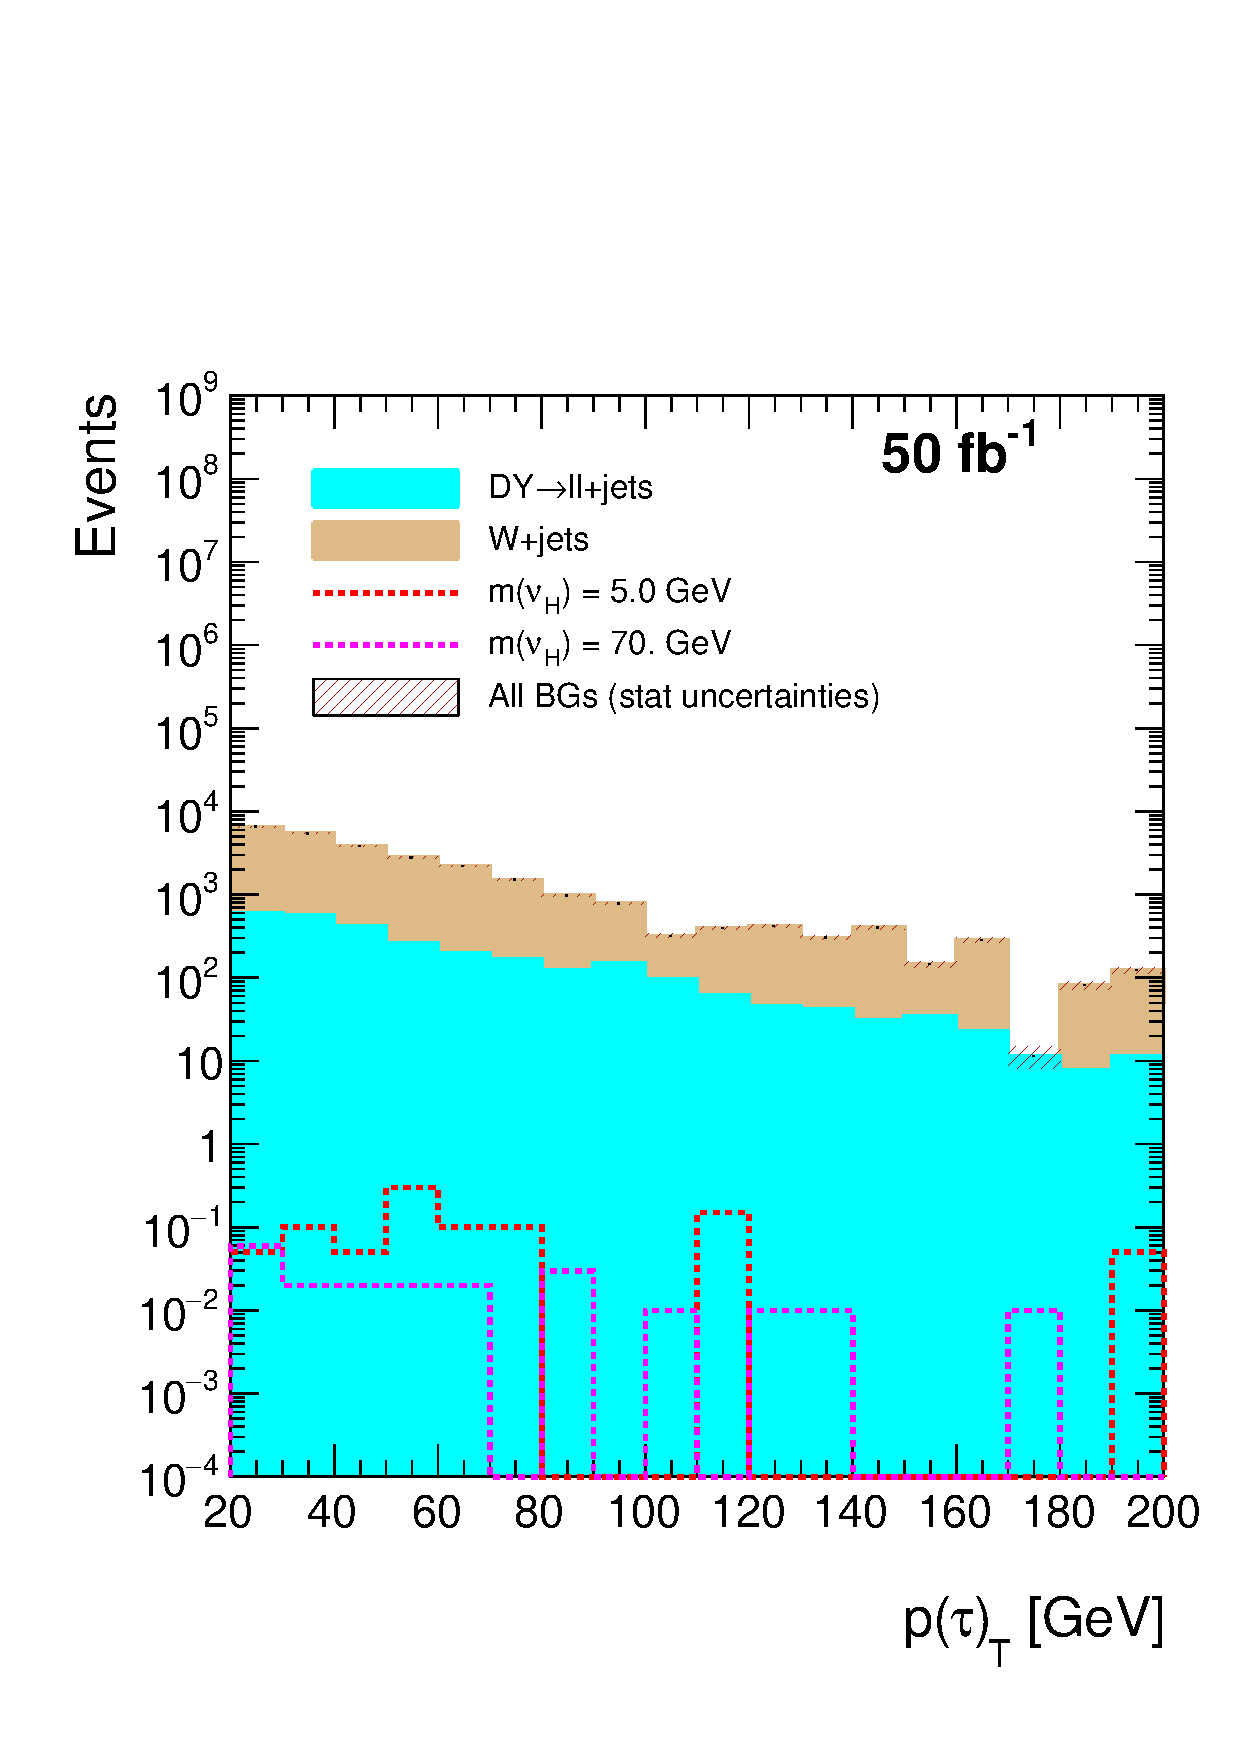
\includegraphics[width=1.1\linewidth]{./Capitulos/Analysis/AfterVBFCUTS/TauPt_MET20}
  \caption{$p_T(\tau)$ distribution for the signal and background}
  \label{taupt_VBF}
\end{subfigure}
\caption{Distribution of diferent variables after all the cuts}
\label{Variables_bjets}
\end{figure}
 
One fact that can explain the reason why the VBF cuts do not allow to reduce significantly the background compared to the signal is the similar values of mass of the Higgs boson and the Z boson.
The production mechanism of a Higgs boson is 
identical to the Z gamma production mechanism because the mass difference between the Higgs boson and the Z boson is just 30 GeV. Thus, the characteristics of the VBF jets in the events are similar
and it is difficult to distinguish both VBF topologies. In the case that the heavy neutrinos are produced by the decay of a particle heavier that the Higgs boson, this heavier particle must be the
result of the interaction of more energetic VBF jets. Thus, in this case it is expected that the detected VBF jets would be more energetic, which would lead to differentiate both final states.

Since it was expected that the resulting tau in the signal had an associated track with a displaced vertex, some 2D plots were made using this variable. First, a graphic on which the x axis 
represents $\vec{E_T^{miss}}$ and the y axis the impact parameter ($d_{xy}$) is shown in the Figure \ref{ipt1_MET}. The two graphics at the left of this figure correspond to the signal events, one 
assuming a mass of the heavy neutrino of 5.0 GeV, and the other of 70.0 GeV. The range of the y axis for both graphics is just from -1.0 to 1.0. The left graphics at the right of the figure correspond 
to the W+jets background and DY+jets background. These graphics have a range in the y axis from -8.0 to 8.0. It can be seen that for our signals the value of the impact parameter is almost zero. 
This implies that it is not possible to make a cut on this variable to reduce the background as it was expected. 
 
 \begin{figure}[h] 
 \centering
 \caption{2D graphic: $E_T^{miss}$ vs $d_{xy}$}
 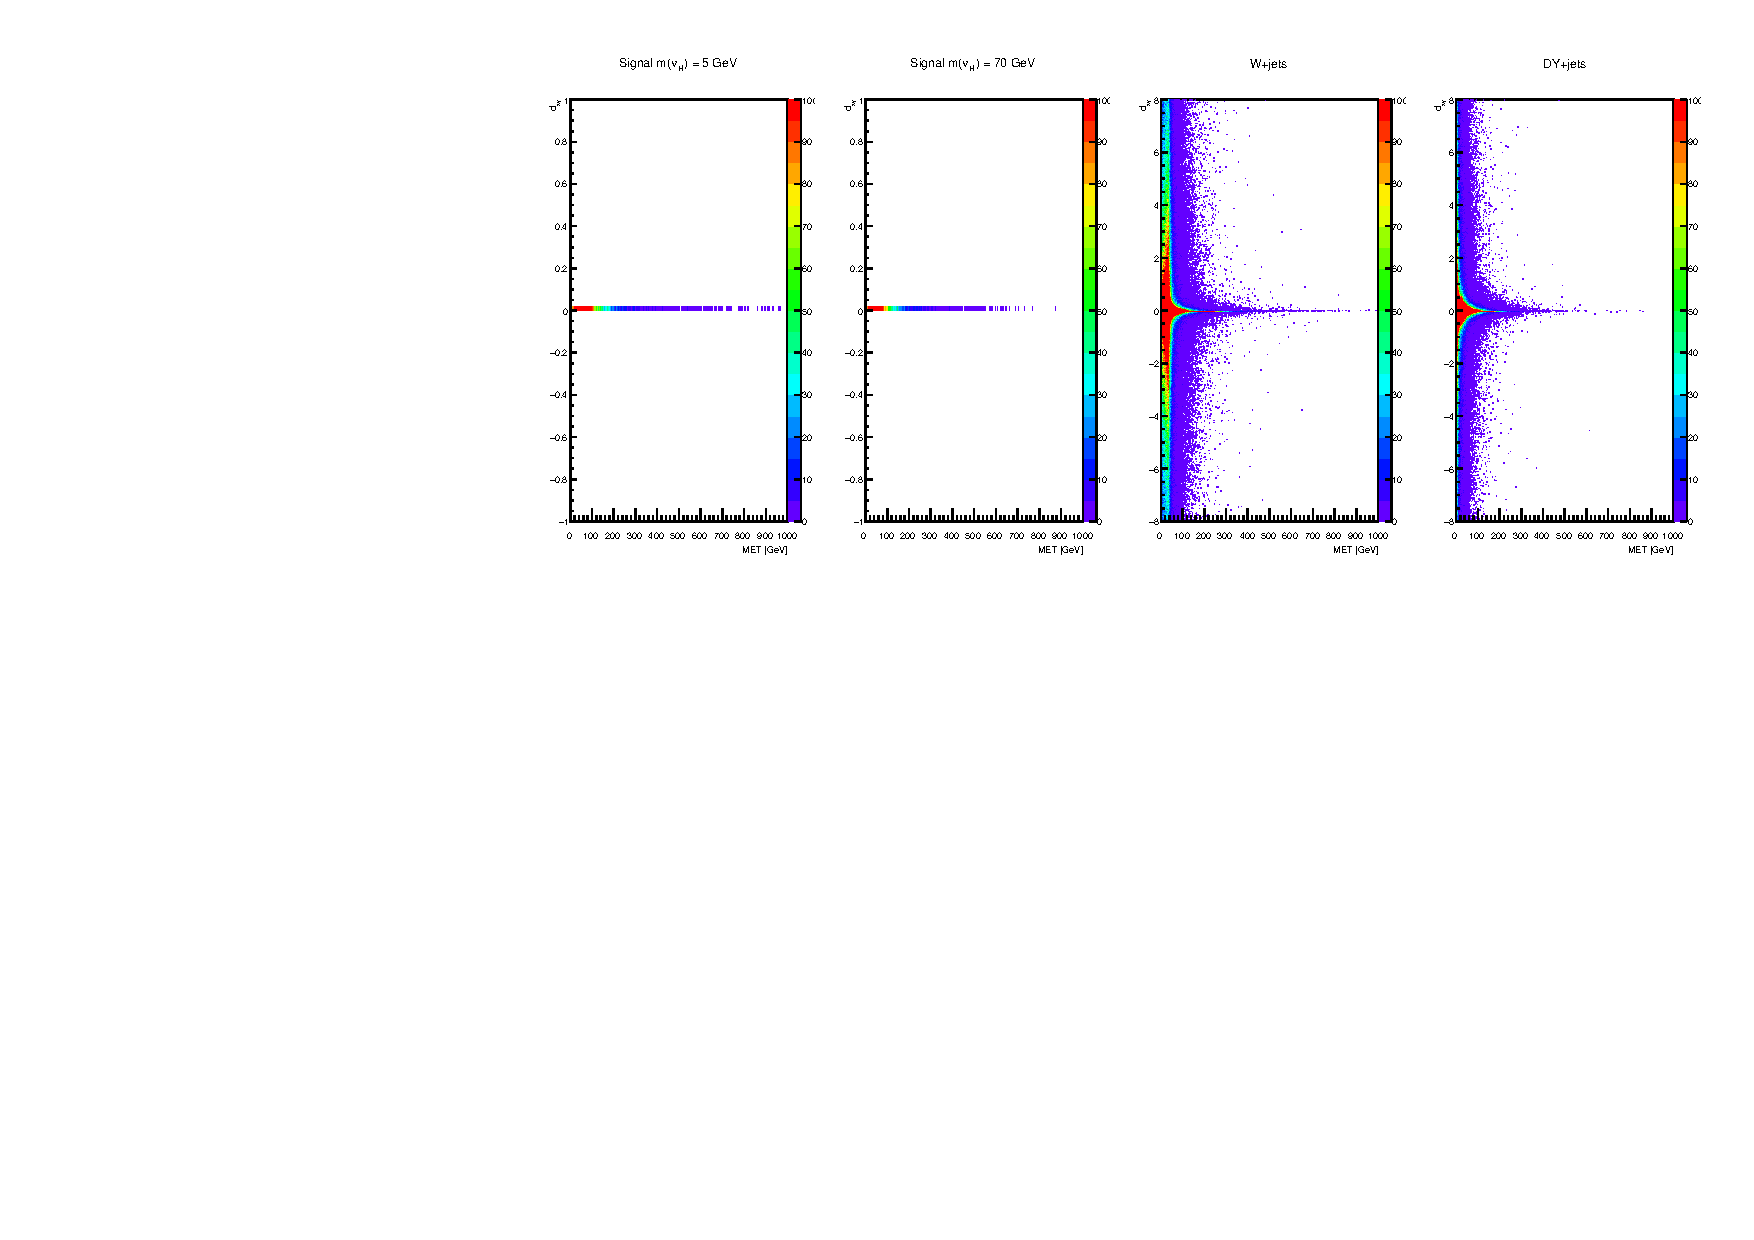
\includegraphics[width=0.8\textwidth]{./Capitulos/Analysis/c1} 
 \label{ipt1_MET}
 \end{figure}
 
 The other 2D graphic studied was 
 
 
 
 